\documentclass{beamer}

\usetheme{Madrid}
\usecolortheme{default}
\usepackage{svg}

\title{IRSE Projecet}
\author{Jan Cichomski (r1026448)}
\date{\today}

\begin{document}

\begin{frame}
  \titlepage
\end{frame}

\begin{frame}{Outline}
  \tableofcontents
\end{frame}
\begin{frame}{TODOS}
  \begin{itemize}
    \item  why have i chose F1 as a metric?
  \end{itemize}
\end{frame}

\begin{frame}{1. Architecture}
  \centering
  \includesvg[width=0.9\textwidth]{architecture.svg}
\end{frame}

\begin{frame}{2. Term Vocabulary}

\end{frame}

\begin{frame}{2.1 Term Vocabulary - Document Preprocessing}
  \begin{itemize}
    \item To lower case
    \item Remove punctuation
    \item Tokenize
    \item Remove english stop words (added custom stop words)
    \item Lemmatize
  \end{itemize}
\end{frame}

\begin{frame}[fragile]{2.1 Temr Vocabulary - Document Preprocessing}
  \begin{verbatim}
def preprocess_text(doc):
    doc = doc.translate(str.maketrans("", "",
        string.punctuation)).lower()
    words = word_tokenize(doc)
    words = [
        lemmatizer.lemmatize(word)
        for word in words
        if word not in stop_words and word.isalpha()
    ]
    return " ".join(words)
    \end{verbatim}
\end{frame}
\begin{frame}[fragile]{2.1 Term Vocabulary - Custom stop words}
  \begin{verbatim}
stop_words.update(
    [
        "add",
        "added",
        "adding",
        "addition",
        "also",
        "almost",
        "another",
        "easily",
        "easy",
    ]
)
    \end{verbatim}
\end{frame}

\begin{frame}{2.2 Term Vocabulary - Hyperparameters}
  Two types of terms:
  \begin{itemize}
    \item 1-grams
          \begin{itemize}
            \item min\_df=20
            \item max\_df=0.5
          \end{itemize}
    \item 2-grams
          \begin{itemize}
            \item 10,000 terms
            \item min\_df=50
            \item max\_df=0.4
          \end{itemize}
  \end{itemize}

\end{frame}

\begin{frame}{2.3 Term Vocabulary - Handling mulit-word terms}
  \begin{itemize}
    \item 2-grams with aggressive filtering
  \end{itemize}
\end{frame}

\begin{frame}{3 Document Embedding}
\end{frame}

\begin{frame}{3.1 Document Embedding - Chosen Fields}
  Fields used for embedding:
  \begin{itemize}
    \item name
    \item description
    \item ingredients
    \item steps
  \end{itemize}

  Evaluated combinations:
  \begin{itemize}
    \item name, description, ingredients, steps: macro F1: 0.126
    \item description, ingredients, steps: macro F1: 0.095
    \item description, ingredients: macro F1: 0.034
    \item description, steps: macro F1: 0.088
    \item description: macro F1: 0.043
  \end{itemize}

\end{frame}

\begin{frame}[fragile]{3.2 Document Embedding - Query Preprocessing}
  The same approche as for embedding documents
  \begin{verbatim}
  def retrieve_documents(query_text, recipies,
                    recipe_ids, k, threshold):
  query = preprocess_text(query_text)
  ...
    \end{verbatim}
\end{frame}

\begin{frame}{3.3 Document Embedding - Edge Cases}
  \begin{itemize}
    \item When query has no terms from vocabulary
          \begin{itemize}
            \item TF-IDF produces zero vector for the query
            \item Cosine similarity returns 0 for all documents
          \end{itemize}
    \item Consequently:
          \begin{itemize}
            \item Without similarity threshold: All documents returned (no filtering)
            \item With any similarity threshold: No documents returned (empty result)
          \end{itemize}
  \end{itemize}
\end{frame}

\begin{frame}{4 Retrieval}
\end{frame}

\begin{frame}{4.1 Retrieval - Similarity Measure}
  \begin{itemize}
    \item Cosine similarity (F1: 0.126) - picked finally
    \item Euclidean distance (F1: 0.064)
  \end{itemize}
\end{frame}

\begin{frame}[fragile]{4.2 Retrieval - Hyperparameters}
  \begin{itemize}
    \item Max number of returned documents: 40
    \item Minimum threshold for cosine similarity: 0.2
  \end{itemize}
  Grid search over param space and maximize macro F1 score.

  \begin{verbatim}
def create_parameter_heatmap(queries, recipes, recipe_ids):
  thresholds = np.arange(0.1, 0.60, 0.05)
  k_values = np.arange(20, 60, 5)
  \end{verbatim}

\end{frame}

\begin{frame}
  \centering
  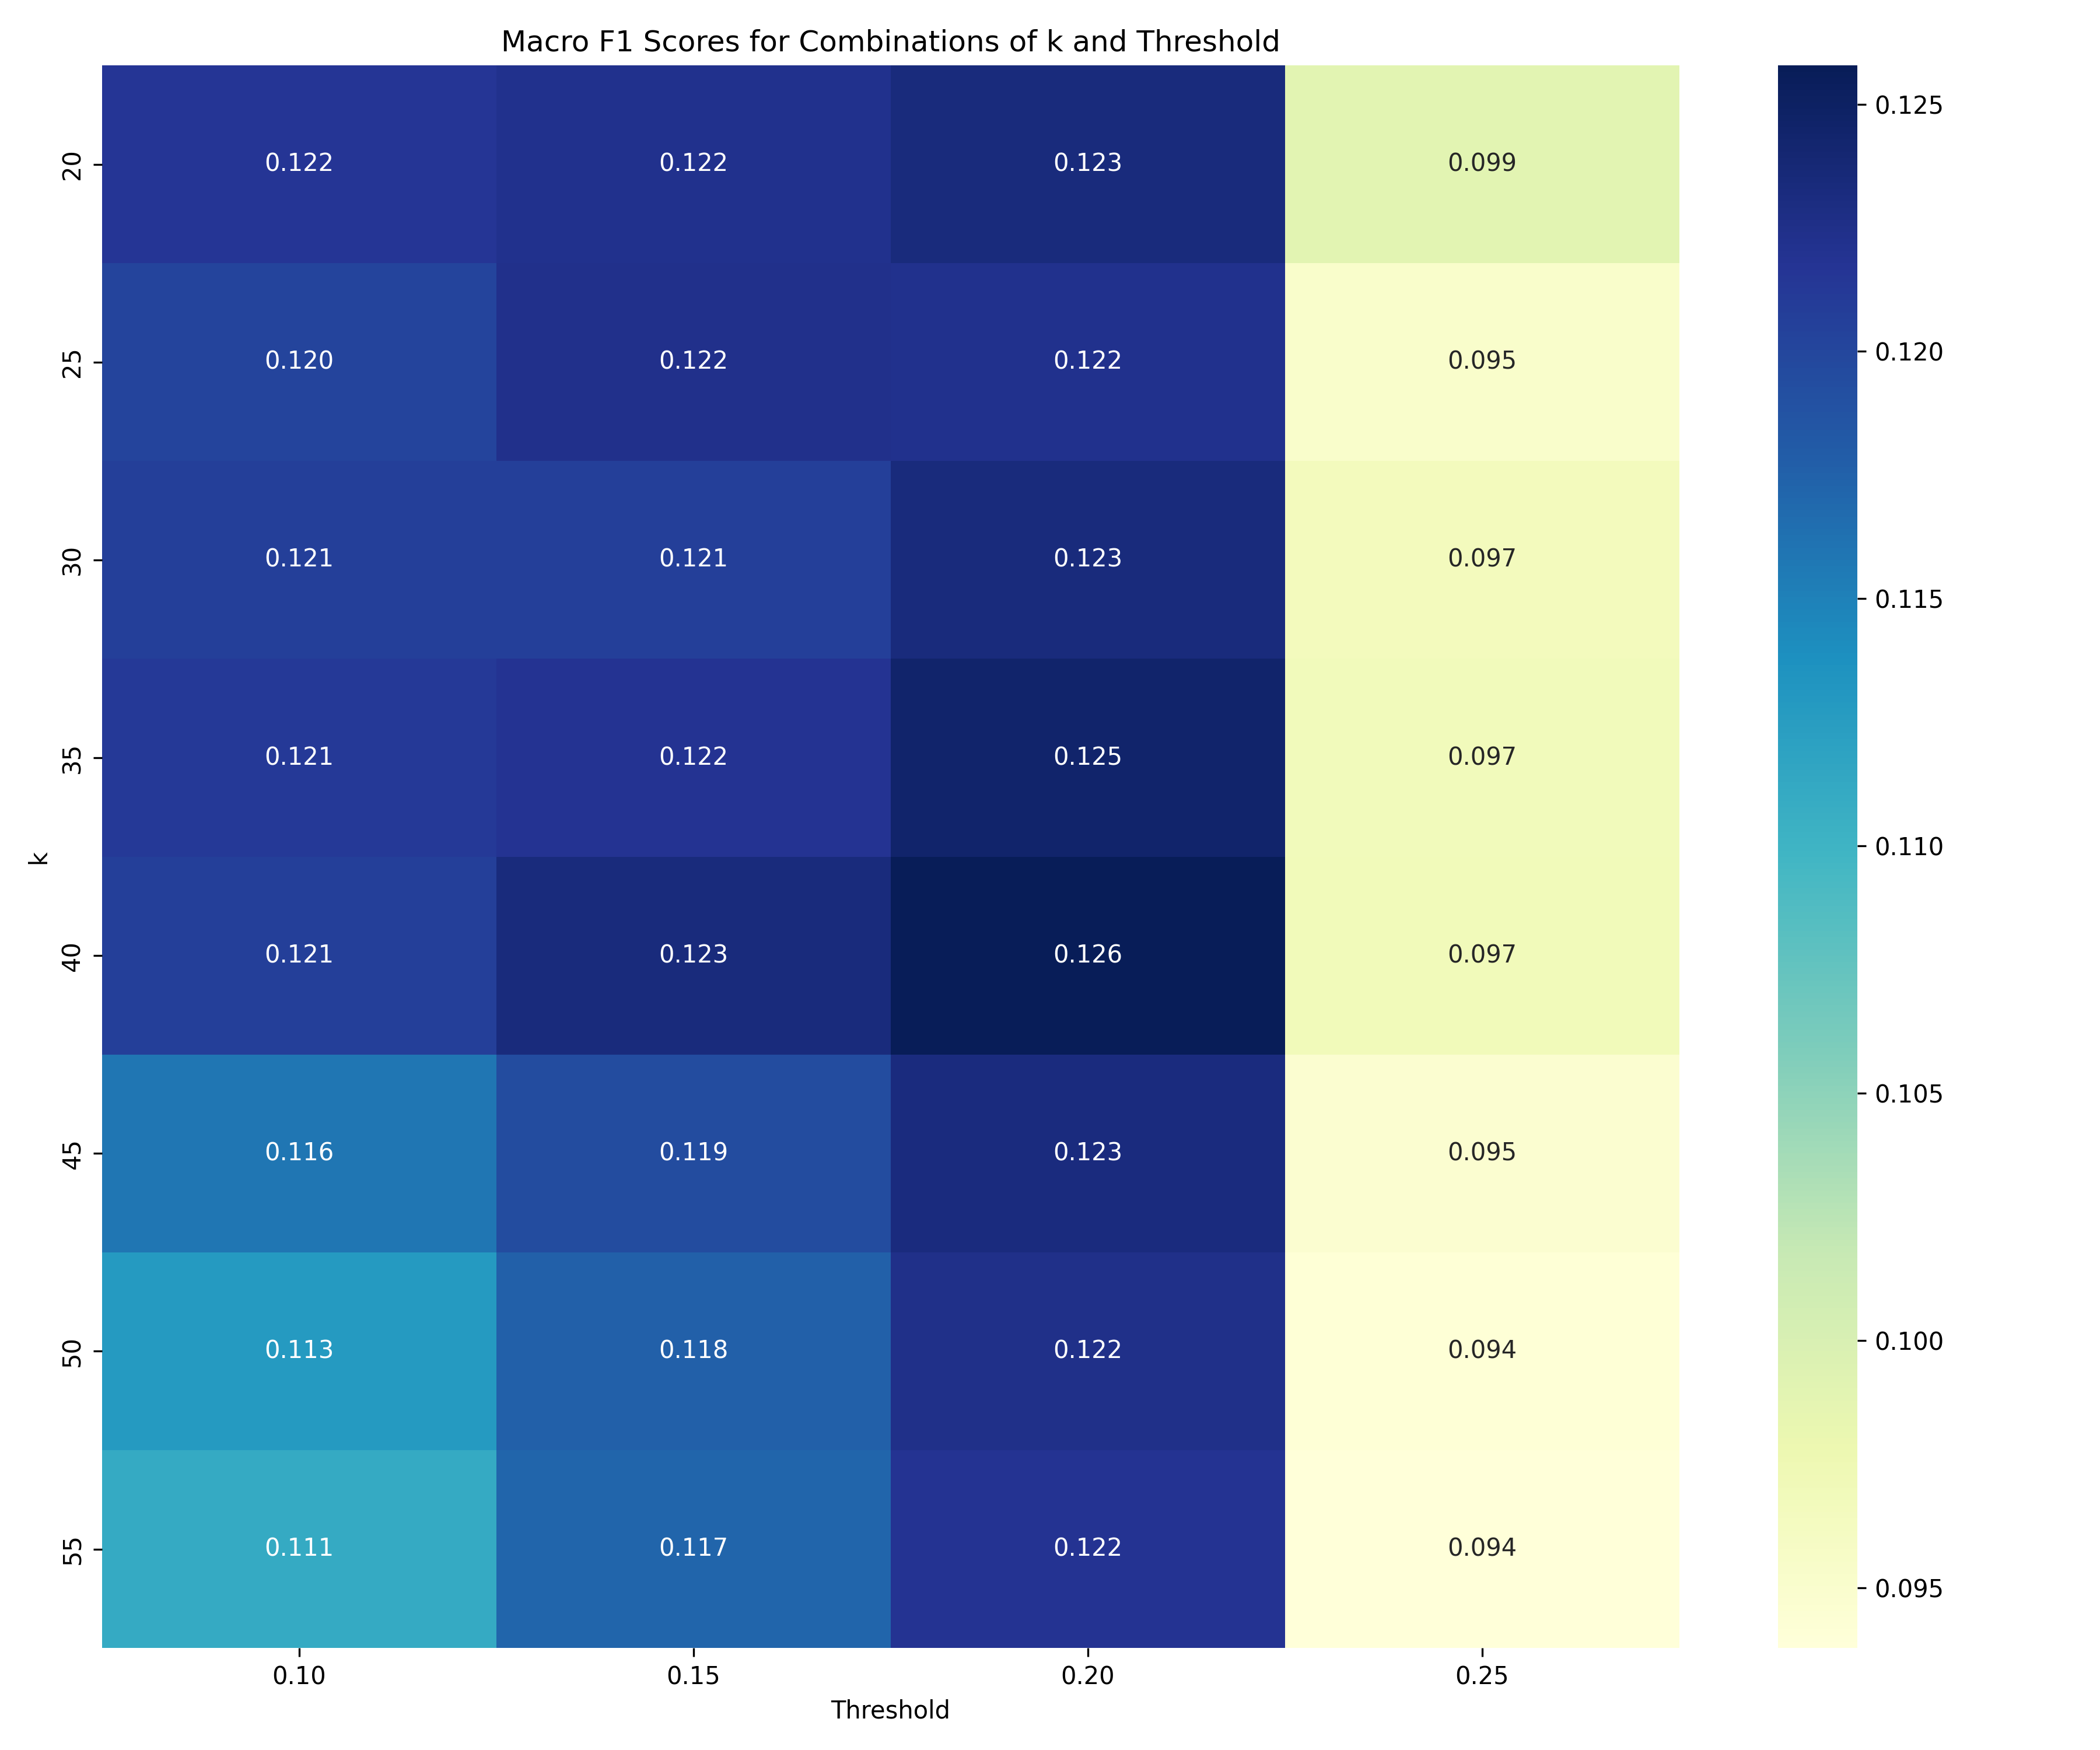
\includegraphics[width=0.9\textwidth]{ir_parameter_heatmap1747239585.png}
\end{frame}

\begin{frame}{4.3 Retrieval - Evaluation Metrics}
  \begin{itemize}
    \item Macro Precision: 0.130
    \item Macro Recall: 0.201
    \item Macro F1: 0.126
    \item Micro Precision: 0.128
    \item Micro Recall: 0.191
    \item Micro F1: 0.153
  \end{itemize}
\end{frame}

\begin{frame}{4.4 Retrieval - MAP}
  Mean Average Precision (MAP): 0.086
  \begin{equation}
    AP = \frac{1}{RD} \sum_{k=1}^{n} P(k) \cdot r(k),
  \end{equation}
  Were $RD$  is the number of relevant documents for the query, $n$ is the total number of documents, $P(k)$
  is the precision at $k$, and $r(k)$ is the relevance of the $k^{th}$ retrieved document ($0$ if not relevant, and $1$ if
  relevant)
  \begin{equation}
    MAP = \frac{1}{Q} \sum_{i=1}^{Q} AP_i
  \end{equation}
  Where $Q$ is the number of queries and $AP_i$ is the average precision for the $i^{th}$ query.
\end{frame}

\begin{frame}[fragile]{4.4 Retrieval - MAP Code}
  \begin{verbatim}
def calculate_average_precision(relevant_doc_ids,
                                retrieved_doc_ids):
  hit_count = 0
  sum_precisions = 0.0
  for i, doc_id in enumerate(retrieved_doc_ids):
      if doc_id in relevant_doc_ids:
          hit_count += 1
          precision_at_i = hit_count / (i + 1)
          sum_precisions += precision_at_i
      # else: sum_precisions += 0.0
  if len(relevant_doc_ids) == 0:
      return 0.0
  return sum_precisions / len(relevant_doc_ids)
  \end{verbatim}
\end{frame}

\begin{frame} {5. Qualitative analysis - Information Retrieval}
  TIODO TODO TODO
\end{frame}

\begin{frame} {5.1 Qualitative analysis - Information Retrieval}
  Problem: Even though there is no relevant information in the document, the system returns some documents\\
  Prompt: "Where can I follow cooking classes"\\
  Output: cinnamon roll glaze taste facs class (0.2410), grandma jayne shrimp dip (0.2369)
\end{frame}

\begin{frame} {5.2 Qualitative analysis - Information Retrieval}
  Problem: Ignores context of entities in query\\
  Prompt: "How does Gordon Ramsay make his beef Wellington?"\\
  Output: Non of the results were about Ramsay making beef wellington
  \begin{table}[]
    \centering
    \begin{tabular}{|l|l|l|l|}
      \hline
      \textbf{ID} & \textbf{Score} & \textbf{Words Contained} & \textbf{Words Not Contained} \\ \hline
      94359       & 0.2972         & ramsay, gordon           & beef, wellington             \\ \hline
      94358       & 0.2502         & ramsay, gordon           & beef, wellington             \\ \hline
      111233      & 0.2448         & beef, wellington         & ramsay, gordon               \\ \hline
      163842      & 0.2439         & beef, wellington         & ramsay, gordon               \\ \hline
      94347       & 0.2207         & ramsay, gordon           & beef, wellington             \\ \hline
      100473      & 0.2146         & beef, wellington         & ramsay, gordon               \\ \hline
      126542      & 0.2086         & beef, wellington         & ramsay, gordon               \\ \hline
      94354       & 0.2069         & ramsay, gordon, beef     & wellington                   \\ \hline
      170428      & 0.2032         & ramsay, gordon           & beef, wellington             \\ \hline
      94353       & 0.2029         & ramsay, gordon           & beef, wellington             \\ \hline
    \end{tabular}
  \end{table}
\end{frame}

\begin{frame} {5.3 Qualitative analysis - Information Retrieval}
  Problem: Can't handle extermalyl rare words, like "Paraguay"\\
  Prompt: "Do you know any soups from Paraguay?"\\
  Output: Did not returned any recipe with word "paraguay"
\end{frame}

\begin{frame} {5.4 Qualitative analysis - Information Retrieval}
  Problem: TF-IDF doesn't handle typos\\
  Prompt: "How do you make \textbf{piza}"\\
  Output: Returned single recipe what contains a lot of words "make", but no "pizza"
\end{frame}

\begin{frame} {5.5 Qualitative analysis - Information Retrieval}
  Problem: Can't capture negation\\
  Prompt:  "I do not want to eat pizza, what can I eat instead?"\\
  Output: 36/40 results were about pizza % and they are about making pizza
\end{frame}

\begin{frame}{6. Prompt}
  Model: mistralai/Mistral-7B-Instruct-v0.2
\end{frame}

\begin{frame}[fragile]{6.1 Prompt - LLM Instructions - Good}
  \begin{itemize}
    \item General context and LLM's goal
    \item Instructions per type of question
    \item Response format
    \item Limitations
  \end{itemize}

  See handout for full prompt
  TODO: add full prompt in handout
\end{frame}

\begin{frame}[fragile]{6.1 Prompt - LLM Instructions - Bad}
  Only general context without specific instructions how to answer the question
  \begin{verbatim}
You are a helpful recipe assistant with access to a database
of recipes. The system has already retrieved the most
relevant recipes to the user's query using TF-IDF similarity.
Your goal is to provide helpful,accurate responses about
recipes, cooking techniques, ingredient substitutions, and
culinary advice based on the retrieved recipes.

The following recipes have been retrieved as most relevant
to the user's query:
{retrieved_recipes}

## User Query
{user_query}
\end{verbatim}
\end{frame}

\begin{frame}{6.2 Prompt - Fields used}
  \begin{itemize}
    \item name
    \item description
    \item ingredients
    \item steps
    \item relevance score
  \end{itemize}
\end{frame}

\begin{frame}[fragile]{6.2 Prompt - Fields used}
  \begin{verbatim}
results = retrieve_documents(query, recipies, recipe_ids, k=k, threshold=threshold)
retrieved_recipes = ""

for idx, (recipe, recipe_id, score) in enumerate(results):
  info=df[df["official_id"] == recipe_id].iloc[0]
  retrieved_recipes+=f"Document {idx}, Score: {score:.4f}\n"
  retrieved_recipes+=f"Name: {info['name']}\n"
  retrieved_recipes+=f"Description:{info['description']}\n"
  retrieved_recipes+=f"Ingredients:{info['ingredients']}\n"
  retrieved_recipes+=f"Steps: {info['steps']}\n\n"

prompt = prompt_template.format(
  retrieved_recipes=retrieved_recipes, user_query=query
)
  \end{verbatim}
\end{frame}

\begin{frame}{7. Qualitative analysis - LLM}
\end{frame}

\begin{frame}{7.1 Qualitative analysis - LLM \& RAG}
  \begin{itemize}
    \item More or less yes
    \item But does not stick to rules
    \item Response are often too general
  \end{itemize}
\end{frame}

% DONE UP TO HERE
\begin{frame}{7.2 Qualitative analysis - LLM Reasoning 1}
  Q: "I'm looking for a spicy pasta sauce, but I forgot the name. I think it was related to Arabs?"
  TODO
\end{frame}

\begin{frame}{7.2 Qualitative analysis - LLM Reasoning 2}
  TODO
\end{frame}

\begin{frame}{7.2 Qualitative analysis - LLM Reasoning 3}
  TODO
\end{frame}

\begin{frame}{7.2 Qualitative analysis - LLM Reasoning 4}
  TODO
\end{frame}

\begin{frame}{7.2 Qualitative analysis - LLM Reasoning 5}
  TODO
\end{frame}


\begin{frame}[fragile]{7.3 Qualitative analysis - Hallucination}
  \begin{itemize}
    \item Standard prompt, but with no documents provided \\
          "How does Gordon Ramsay make his beef Wellington?"
    \item Yet LLM answered with recipe
    \item Which suggest that it did not followed rules
  \end{itemize}
  \begin{verbatim}
The following recipes have been retrieved as most relevant
to the user's query:

## Instructions

{rest of the prompt}

[/INST] Based on the retrieved recipes, Gordon Ramsay's Beef
Wellington is typically made with a large piece of beef
fillet, duplicated with a sheet of pate, covered in
mushrooms and pastry, and baked in an oven.
...
  \end{verbatim}
\end{frame}

\begin{frame}{7.4 Qualitative analysis - Score vs No Score - TODO }
\end{frame}

\begin{frame}{8. Neural document embeddings}
\end{frame}

\begin{frame}[fragile]{8.1 Neural document embeddings - out of vocabulary - query}
  Used model's tokenizer to tokenize the query
  \begin{itemize}
    \item Original text: 'kashubian'
    \item \begin{verbatim}[CLS]', 'ka', '##shu', '##bian', '[SEP]'\end{verbatim}
  \end{itemize}
  The \verb|##| prefix represents subword tokenization, allowing the model to handle words not in its vocabulary.
\end{frame}
\begin{frame}[fragile]{8.1 Neural document embeddings - out of vocabulary - document}
  Used model's tokenizer to tokenize the query
  \begin{itemize}
    \item Original text: 'their settlement area is referred to as kashubia they speak the kashubian language which is classified either...'
    \item \begin{verbatim}
'[CLS]', 'their', 'settlement', 'area', 'is', 'referred',
'to', 'as', 'ka', '##shu', '##bia', 'they', 'speak',
'the', 'ka', '##shu', '##bian', 'language', 'which',
'is', 'classified', 'either',\end{verbatim}
  \end{itemize}
  Neural embeddings returned valid results even through the word "kashubian" was not in the vocabulary.
\end{frame}

\begin{frame}{8.2 Neural document embeddings - Metrics - Recipes}
  \begin{itemize}
    \item Macro Precision: 0.307
    \item Macro Recall: 0.134
    \item Macro F1: 0.157
    \item Micro Precision: 0.280
    \item Micro Recall: 0.035
    \item Micro F1: 0.062
    \item MAP: 0.101
    \item Average DCG: 2.472
    \item Average NDCG: 0.736
  \end{itemize}
\end{frame}

\begin{frame}{8.2 Neural document embeddings - Metrics - Wiki}
  \begin{itemize}
    \item Macro Precision: 0.310
    \item Macro Recall: 0.352
    \item Macro F1: 0.260
    \item Micro Precision: 0.343
    \item Micro Recall: 0.303
    \item Micro F1: 0.322
    \item MAP: 0.216
    \item Average DCG: 1.566
    \item Average NDCG: 0.549
  \end{itemize}
\end{frame}

\begin{frame}{9. Compression}
\end{frame}

\begin{frame}{9.1 Compression - Long Dcouments}
  Information Retrieval
  \begin{itemize}
    \item Cover multiple topics
    \item Contain lots of words
    \item Limited document length
  \end{itemize}
  LLM
  \begin{itemize}
    \item Limited context widnow
    \item Needle in a haystack
  \end{itemize}
\end{frame}

\begin{frame}[fragile]{9.2 Compression - Solutoin}
  Split documents into chunks
  \begin{verbatim}
from langchain_text_splitters
  import RecursiveCharacterTextSplitter
text_splitter = RecursiveCharacterTextSplitter(
  chunk_size=500,
  chunk_overlap=100,
  length_function=len,
  is_separator_regex=False,
)
\end{verbatim}
\end{frame}

\begin{frame}{9. Security}
\end{frame}

\begin{frame}{9.1 Security}
  \begin{itemize}
    \item Yes, LLM is susectipble TODO...
  \end{itemize}
\end{frame}

\end{document}